\nxsection{Le R\^ole ''Caissier''}\label{sec:utilisateurs-lecaissier}
\index{caissier}
\index{LeCaissier}

La figure~\ref{fig:fenetre-principale-caissier} illustre la
fen\^etre d'acceuil d'un utilisateur avec le \role \caissier,
apr\`es qu'il se soit enregistr\'e dans \yeren.\\

\begin{figure}[!htbp]
\centering
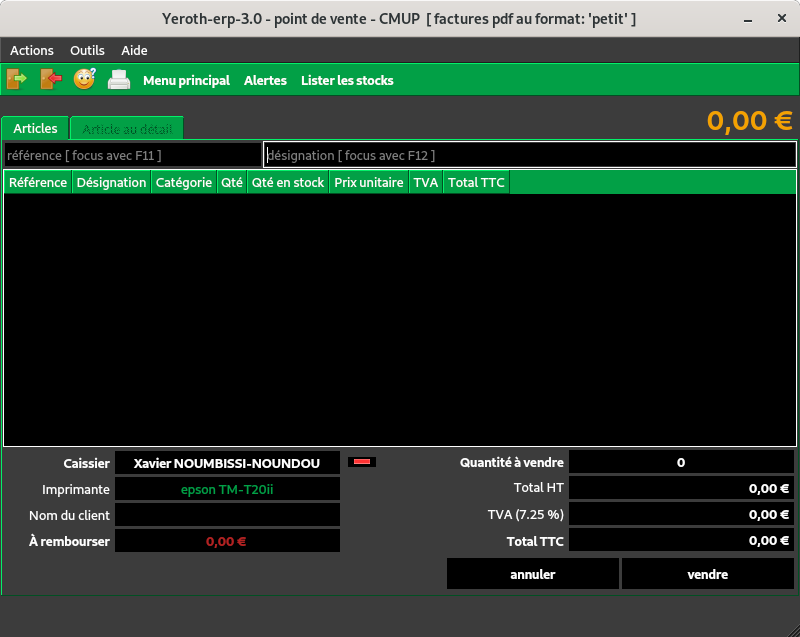
\includegraphics[scale=0.63]{images/yeren-fenetre-caissier.png}
\caption{La fen\^etre d'acceuil d'un \caissier.}
\label{fig:fenetre-principale-caissier}
\end{figure}

Un utilisateur de \yeren avec le \role \caissier a acc\`es
aux fonctionnalit\'es suivantes:

\begin{enumerate}[1)]
	\item point de vente (voir chapitre~\ref{chap:vendre})
	\item syst\`eme d'alertes (voir chapitre~\ref{chap:systeme-dalertes}).\\
\end{enumerate}